% Uncomment this to make slides with overlays:
%\documentclass[slides]{beamer}

% Uncomment these (but comment the above \documentclass line) to make handouts:
\documentclass[handout]{beamer}

% Uncomment these to have more than one slide per page
%\usepackage{pgfpages}
%\pgfpagesuselayout{2 on 1}[border shrink=5mm]
%\pgfpageslogicalpageoptions{1}{border code=\pgfusepath{stroke}}
%\pgfpageslogicalpageoptions{2}{border code=\pgfusepath{stroke}}

\usepackage[]{graphicx, color, hyperref}

\mode<presentation>
{
	%\usetheme[secheader]{Boadilla}
	%\usecolortheme[rgb={.835, .102,.169}]{structure}  
	\usetheme[width= 0cm]{Goettingen}
	%\setbeamercovered{transparent}
}
\setbeamertemplate{navigation symbols}{}
\setbeamertemplate{footline}[frame number]

\definecolor{blue2}{rgb}{0.278,0.278,0.729} 
\newcommand{\blue}[1]{\textcolor{blue2}{#1}}
\newcommand{\white}[1]{\textcolor{white}{#1}}
\newcommand{\red}[1]{\textcolor{red}{#1}}
\newcommand{\xbar}{\overline{x}}
\newcommand{\ybar}{\overline{y}}
\newcommand{\phat}{\widehat{p}}
\newcommand{\prob}{\mbox{Pr}}
\newcommand{\E}{\mathbb{E}}
\newcommand{\Var}{\mbox{Var}}
\newcommand{\cp}{\oplus}
\newcommand{\cm}{\circleddash}


\title{Lecture 19: ANOVA Part I}
\author{Chapter 5.5}
\date{}


\begin{document}
%------------------------------------------------------------------------------
\begin{frame}
\titlepage
\end{frame}
%------------------------------------------------------------------------------


%-------------------------------------------------------------------------------
\begin{frame}
\frametitle{Previously... Conditions/Assumption for Using t Dist'n}
The key situation to use the $t$ distribution is when you have a \blue{small sample}.

\begin{itemize}
\item \blue{Independence of observations}: To ensure this, either
\begin{itemize}
\item collect a simple random sample that is less than 10\% of the population
\item or if it was an experiment or random process check that each observation was independent
\end{itemize}
\item \blue{Observations come from a nearly normal distribution}:  This second condition is difficult to verify with small data sets:
\begin{itemize}
\item take a look at a plot of the data for obvious departures from the normal model
\item consider whether any previous experiences alert us that the data may not be nearly normal
\end{itemize}
\end{itemize}  	
\end{frame}
%-------------------------------------------------------------------------------



%-------------------------------------------------------------------------------
\begin{frame}
\frametitle{Previously... Confidence Intervals and $t$-Test}

We have the same two methods for inference as in Chapter 4, but:
\begin{enumerate}
\item Confidence intervals:  Now we use $t^*_{df}$ instead of $z^*$
\[
\left[\xbar - t_{df}^* SE, \mbox{  }\xbar + t_{df}^* SE\right] = 
\left[
\overline{x} - t_{df}^* \times\frac{s}{\sqrt n}, \mbox{  }
\overline{x} + t_{df}^* \times\frac{s}{\sqrt n}
\right]
\]
\item Hypothesis testing:  Now we use the \blue{t-test}
\[
t = \frac{\overline{x}-\mbox{null value}}{SE}
\]
using the t-table on page 410 (instead of z-table) for $df=n-1$
\end{enumerate}

\end{frame}
%-------------------------------------------------------------------------------


%------------------------------------------------------------------------------
\begin{frame}[fragile]
\frametitle{New Topic: Analysis of Variance (ANOVA)}
A farmer has the choice of four tomato fertilizers and wants to compare their performance in terms of crop yield.

\pause \vspace{0.5cm}

We have $k=4$ groups AKA \blue{levels of a factor}: the 4 types of fertilizer.  \pause Say we:
\begin{itemize}
\pause \item assign $n_i$ plants to each of the $k=4$ fertilizers as follows:
\[
\begin{array}{cccc|c}
n_1 & n_2 & n_3 & n_4 &\mbox{total }n\\
\hline
3 & 7 & 4 & 6 & 20
\end{array}
\]
\pause \item we evaluate the number of tomatoes on each plant
\end{itemize}

\end{frame}
%------------------------------------------------------------------------------


%%------------------------------------------------------------------------------
%\begin{frame}[fragile]
%\frametitle{New Topic: Analysis of Variance (ANOVA)}
%We use ANOVA to analyze \blue{differences in means} $\mu_1, \ldots, \mu_k$ for $k$ different groups.  Ex: consider the 4 fertilizers and count the number of tomatoes for different plants in two situations:
%
%\begin{center}
%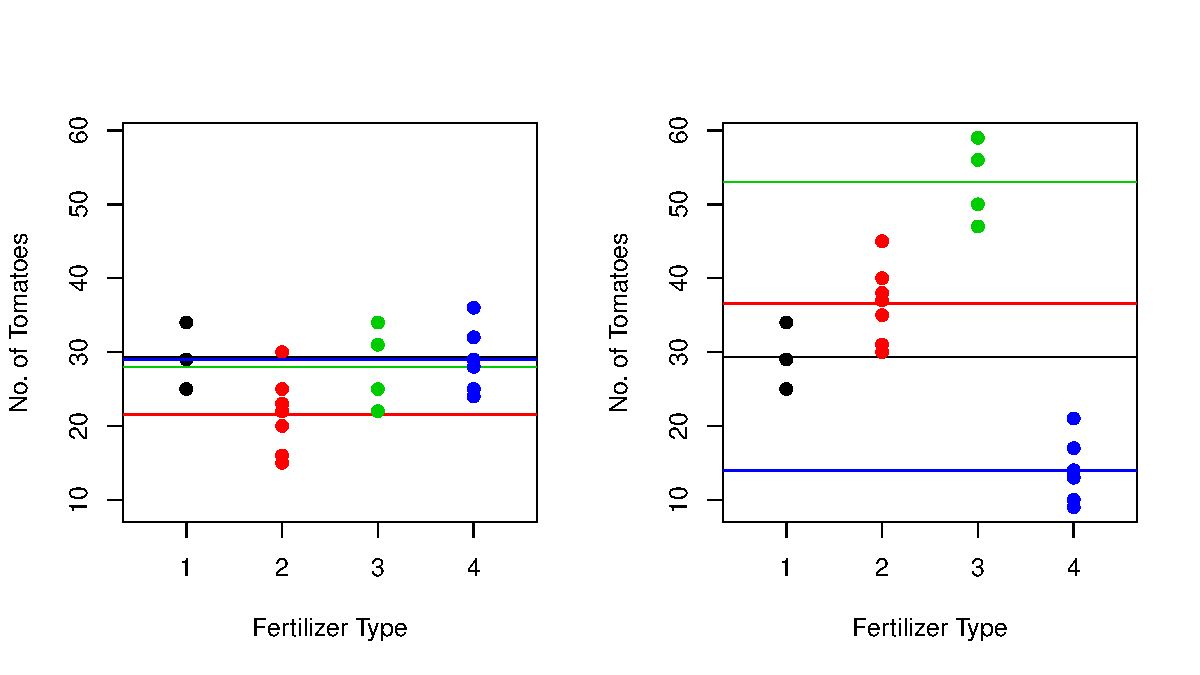
\includegraphics[width=\textwidth]{figure/lec22-007.pdf}
%\end{center}
%
%\end{frame}
%%------------------------------------------------------------------------------


%-------------------------------------------------------------------------------
\begin{frame}
\frametitle{Tomato Fertilizer}
We observe the following data, where each point is one tomato plant. \textcolor{white}{Plot the sample mean of each level.} \textcolor{white}{Question: are the mean tomato yields different?}  
\setkeys{Gin}{width=0.65\textwidth}
\begin{center}
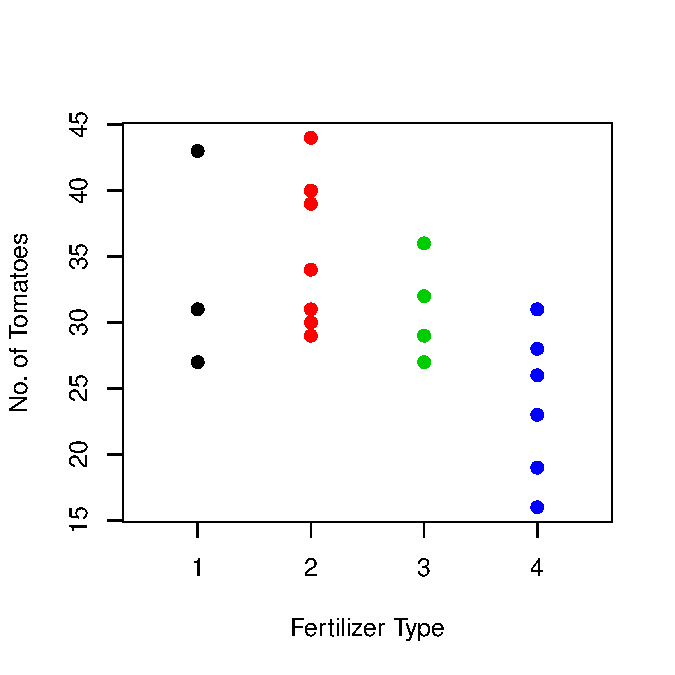
\includegraphics{figure/lec22-003}
\end{center}
\end{frame}
%-------------------------------------------------------------------------------


%-------------------------------------------------------------------------------
\addtocounter{framenumber}{-1}
\begin{frame}
\frametitle{Tomato Fertilizer}
We observe the following data, where each point is one tomato plant.  Plot the sample mean of each level. \textcolor{white}{Question:  are the mean tomato yields different?} 
\setkeys{Gin}{width=0.65\textwidth}
\begin{center}
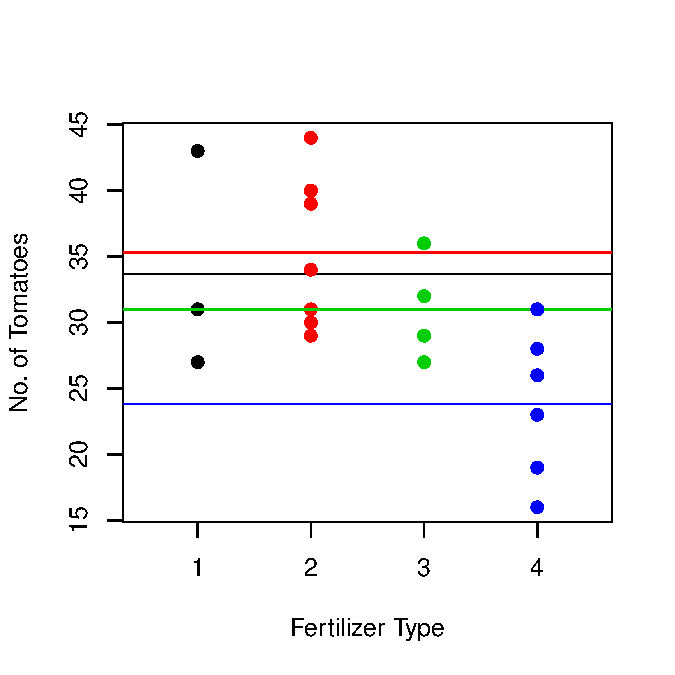
\includegraphics{figure/lec22-004}
\end{center}
\end{frame}
%-------------------------------------------------------------------------------


%-------------------------------------------------------------------------------
\addtocounter{framenumber}{-1}
\begin{frame}
\frametitle{Tomato Fertilizer}
We observe the following data, where each point is one tomato plant.  Plot the sample mean of each level. \blue{Question:  are the mean tomato yields different?}
\setkeys{Gin}{width=0.65\textwidth}
\begin{center}
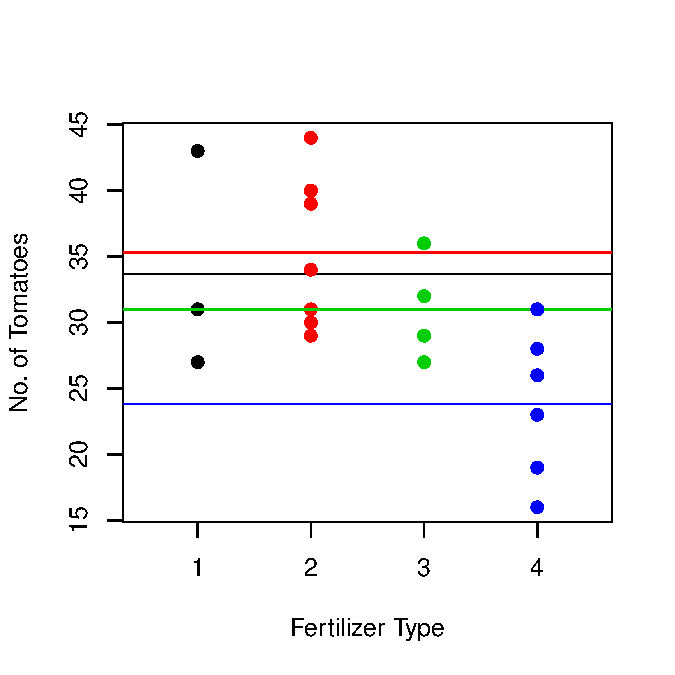
\includegraphics{figure/lec22-004}
\end{center}
\end{frame}
%-------------------------------------------------------------------------------


%-------------------------------------------------------------------------------
\begin{frame}
\frametitle{Analysis of Variance}
Say we have $k$ groups and want to compare the $k$ means:
\[
\mu_1 \mbox{ and } \mu_2 \mbox{ and } \ldots \mbox{ and } \mu_k
\]

\pause \vspace{0.5cm}

We could do ${k \choose 2}$ individual two-sample tests.  Ex. for groups 1 \& 2:
\begin{eqnarray*}
H_0: && \mu_1 = \mu_2\\
\mbox{vs. } H_a:  && \mu_1 \neq \mu_2
\end{eqnarray*}
\pause i.e. no difference in means

\end{frame}
%-------------------------------------------------------------------------------


%-------------------------------------------------------------------------------
\begin{frame}
\frametitle{Analysis of Variance}
Or, rather than conducting all ${k \choose 2}$ tests, we do \blue{a single overall test} via \blue{Analysis of Variance ANOVA}:

\vspace{0.5cm}

\pause The hypothesis test is:
\begin{eqnarray*}
H_0: && \mu_1 = \mu_2 = \ldots = \mu_k\\
\mbox{vs. } H_a:  && \mbox{at least one of the $\mu_i$'s are different}\\
\end{eqnarray*}
\end{frame}
%-------------------------------------------------------------------------------


%-------------------------------------------------------------------------------
\begin{frame}
\frametitle{How ANOVA Tests Work}
ANOVA asks:  where is the overall variability of the data originating from?

\vspace{0.5cm}

\pause The \blue{test statistic} used to compute a $p$-value is now the \blue{F-statistic}:
\[
F = \frac{\mbox{measure of between-group variability}}{\mbox{measure of within-group variability}}
\]
\end{frame}
%-------------------------------------------------------------------------------


%-------------------------------------------------------------------------------
\begin{frame}
\frametitle{Tomato Fertilizer Example}
Numerator: the \blue{between-group variation} refers to the variability \blue{between} the levels (the 4 horizontal lines):  
\setkeys{Gin}{width=0.65\textwidth}
\begin{center}
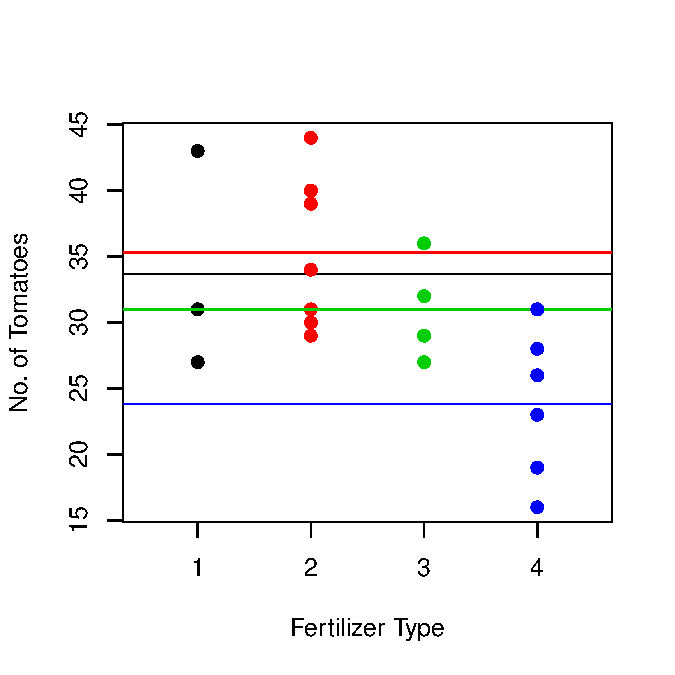
\includegraphics{figure/lec22-006}
\end{center}
\end{frame}
%-------------------------------------------------------------------------------


%-------------------------------------------------------------------------------
\begin{frame}
\frametitle{Tomato Fertilizer Example}
Denominator: the \blue{within-group variation} refers to the variability \blue{within} each level (the 4 vertical arrows):
\setkeys{Gin}{width=0.65\textwidth}
\begin{center}
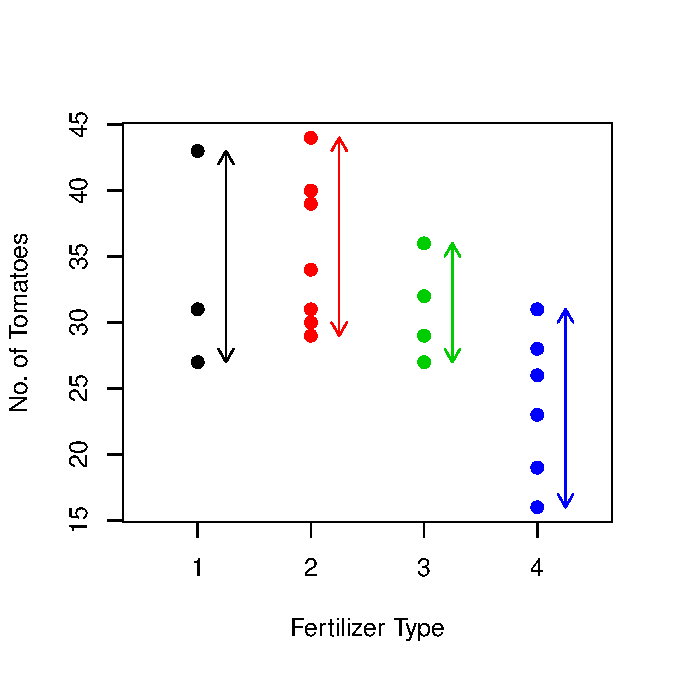
\includegraphics{figure/lec22-005}
\end{center}
\end{frame}
%-------------------------------------------------------------------------------


%-------------------------------------------------------------------------------
\begin{frame}
\frametitle{Tomato Fertilizer Example}
Now compare the following two plots:
\setkeys{Gin}{width=0.8\textwidth}
\begin{center}
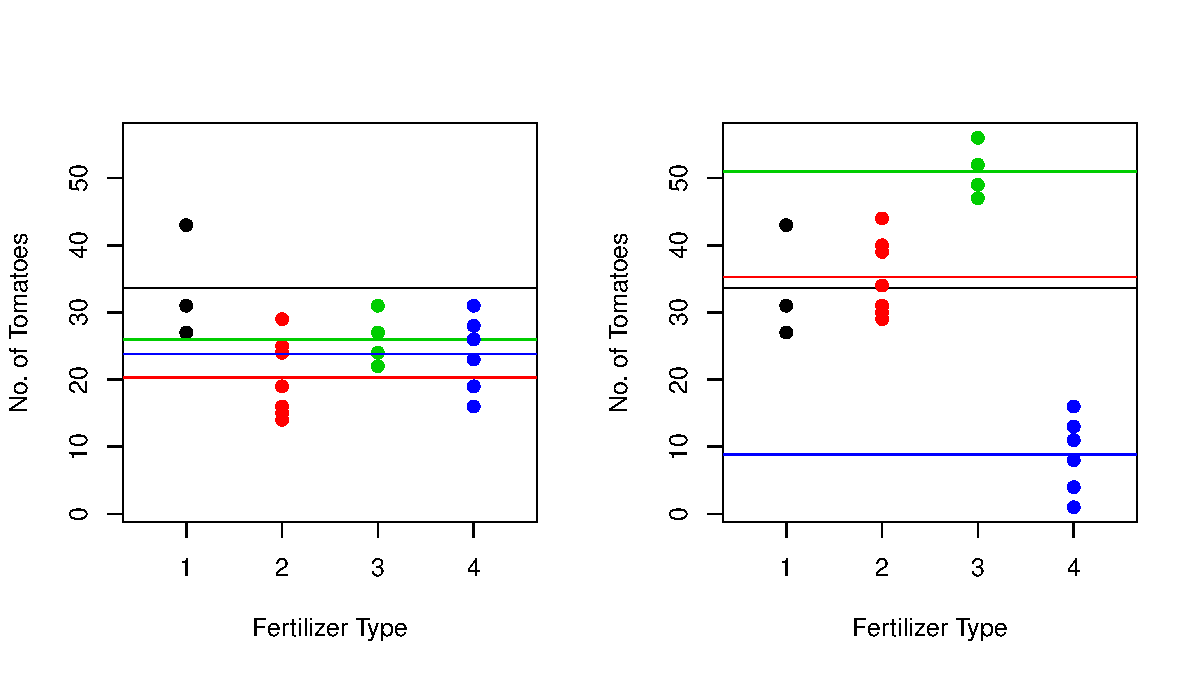
\includegraphics{figure/lec22-008}
\end{center}

\begin{itemize}
\pause \item They have the \blue{same within-group} variability.  Call this value $W$
\pause \item The right plot has \blue{higher between group variability}  b/c the 4 means are more different.  Call these values $B_{left}$ and $B_{right}$ with $B_{left} < B_{right}$
\end{itemize}

\end{frame}
%-------------------------------------------------------------------------------


%-------------------------------------------------------------------------------
\begin{frame}
\frametitle{Tomato Fertilizer Example}
\setkeys{Gin}{width=0.8\textwidth}
\begin{center}
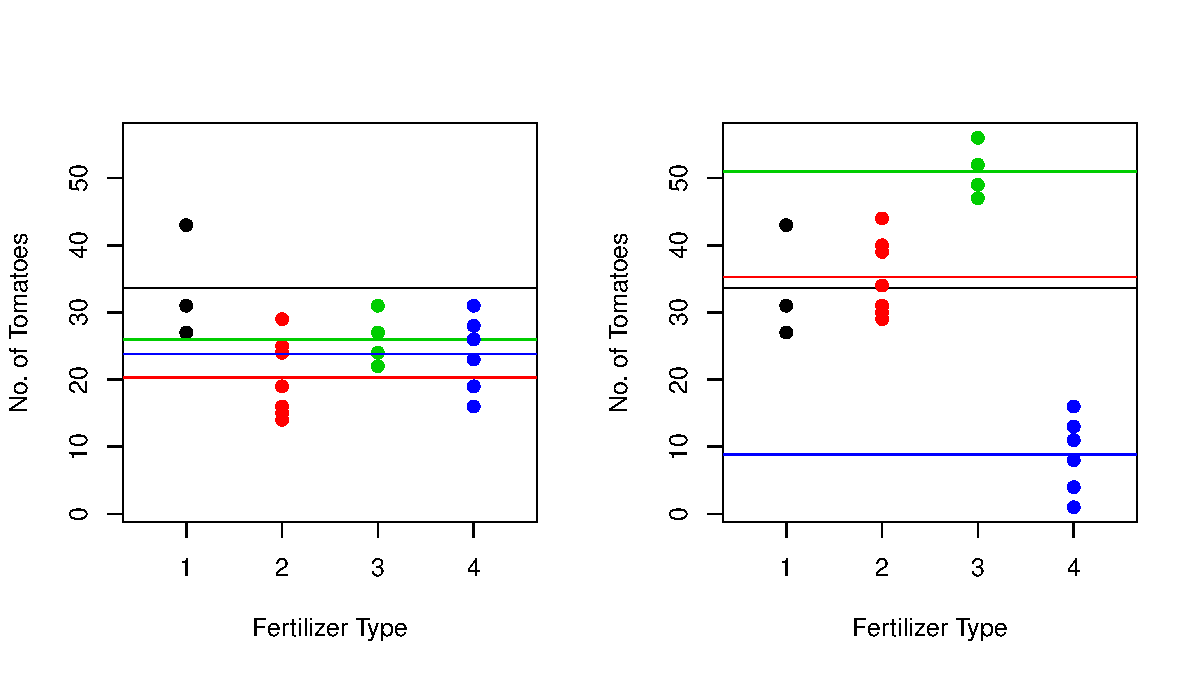
\includegraphics{figure/lec22-008}
\end{center}
\[
\pause \mbox{Recall }F = \frac{\mbox{measure of between-group variability}}{\mbox{measure of within-group variability}} 
\]
\pause \begin{eqnarray*}
\mbox{Since \ }\frac{B_{left}}{W} &<& \frac{B_{right}}{W}\\
\mbox{thus \ \ \  }F_{left} &<& F_{right}
\end{eqnarray*}

\end{frame}
%-------------------------------------------------------------------------------\


%-------------------------------------------------------------------------------
\begin{frame}
\frametitle{$F$ Distributions}
\blue{Assuming $H_0$ is true} (that $\mu_1 = \mu_2 = \ldots = \mu_k$), the $F$-statistic
\[
F = \frac{\mbox{measure of between-group variability}}{\mbox{measure of within-group variability}}
\]
follows the \blue{$F$ distribution with degrees of freedom $df_1=k-1$ and $df_2=n-k$} where
\begin{itemize}
\pause \item $n$ is the \blue{total} number of observations
\item $k$ is the number of groups
\end{itemize}
 
\end{frame}
%-------------------------------------------------------------------------------


%-------------------------------------------------------------------------------
\begin{frame}
\frametitle{$F$ Distributions}
Much like the $t$ distribution with degrees of freedom $df$, the parameters for the $F$ distribution are $df_1=k-1$ and $df_2=n-k$.  Example with $df_1 = 4$ and $df_2=6$:
\setkeys{Gin}{width=0.65\textwidth}
\begin{center}
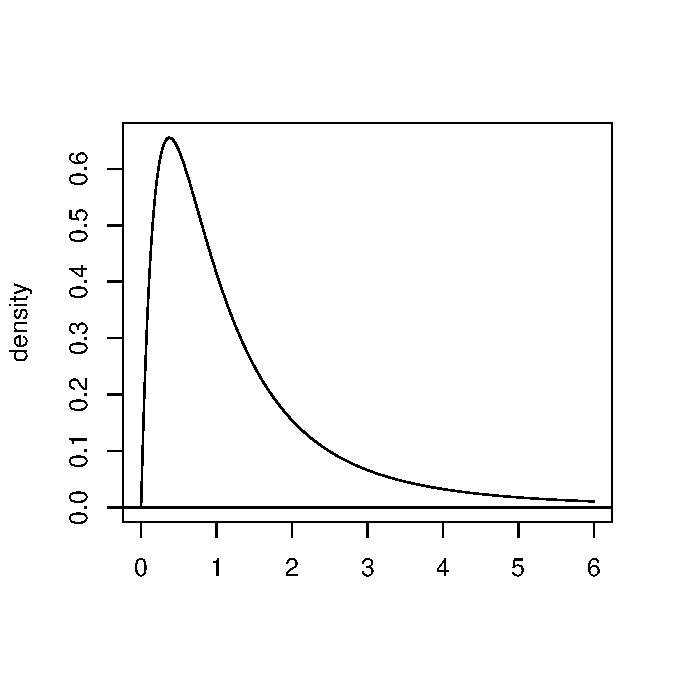
\includegraphics{figure/lec22-009}
\end{center}
\end{frame}
%-------------------------------------------------------------------------------


%-------------------------------------------------------------------------------
\begin{frame}
\frametitle{$F$ Distributions}
$p$-values are computed as before where ``more extreme'' means \blue{larger}.  You can compute these in {\tt R} using {\tt pf(F,df1,df2)}.  Say the $F$-statistic is equal to $3$, the $p$-value is the \blue{area to the right of 3}.
\setkeys{Gin}{width=0.65\textwidth}
\begin{center}
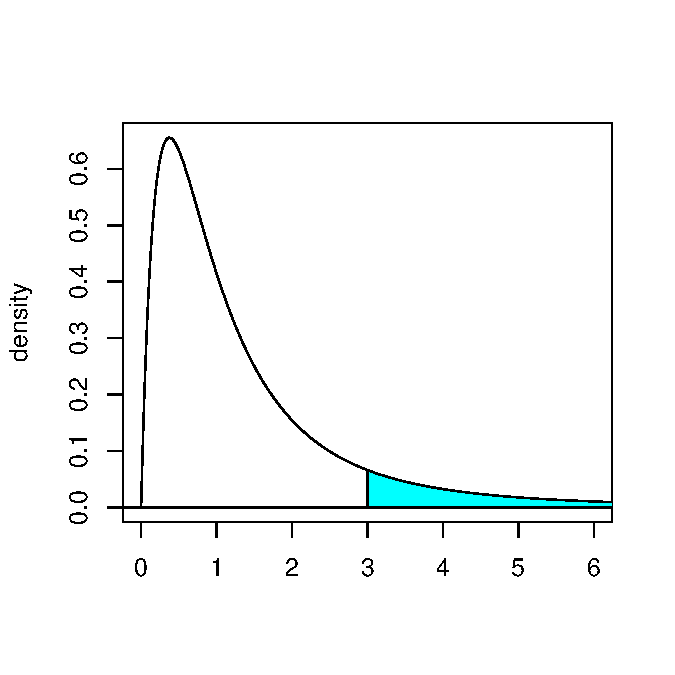
\includegraphics{figure/lec22-010}
\end{center}
\end{frame}
%-------------------------------------------------------------------------------


%-------------------------------------------------------------------------------
\begin{frame}
\frametitle{Conducting An $F$-Test}
The results are typically summarized in an \blue{ANOVA table}:

\begin{small}
\begin{center}
\begin{tabular}{l|ccc|cc}
Source of Variation & $df$ & $SS$ & $MS$ & $F$ & $p$-value\\
\hline
Between groups & $k-1$ & $SSTr$ & $MSTr = \frac{SSTr}{k-1}$ & $\frac{MSTr}{MSE}$ & $p$\\
Within groups & $n-k$ & $SSE$ & $MSE = \frac{SSE}{n-k}$ & & \\
\hline
Total & $n-1$ & $SST$ &  & & 
\end{tabular}
\end{center}
\end{small}
\end{frame}
%-------------------------------------------------------------------------------


%-------------------------------------------------------------------------------
\begin{frame}
\frametitle{Conditions}
\begin{enumerate}
\pause \item The observations have to be \blue{independent}.  10\% rule.  
\pause \item If the sample sizes are small within each group, \blue{normality} of the data is important.  If not small, we can be lax about this. 
\pause \item Each of the groups has \blue{constant variance} $\sigma_1^2 = \ldots = \sigma_k^2 = \sigma^2$.  We can check this with boxplots and by comparing the sample standard deviations $s_1, \ldots, s_k$
\end{enumerate}

\end{frame}
%-------------------------------------------------------------------------------


\end{document}










